\section{Evaluation}
\label{sec.evaluation}

\begin{table*}[!ht]
\begin{tabular*}{\textwidth}{l @{\extracolsep{\fill}} cccc}
\toprule
\multicolumn{5}{c}{Possibility of Triggering Kernel Vulnerabilities} \\
\midrule
Vulnerability    &  Native Linux OS  &  Lind  &  Graphene & VirtualBox\\
\midrule
 CVE-2014-9529 \cite{CVE:20149529} & \ding{55} & \ding{55} & \ding{55} & \ding{55} \\
 CVE-2014-3631 \cite{CVE:20143631} & \ding{55} & \ding{55} & \ding{55} & \ding{55} \\
 CVE-2012-6657 \cite{CVE:20126657} & \ding{55} & \ding{55} & \ding{55} & \ding{55} \\
 CVE-2014-5207 \cite{CVE:20145207} & \ding{55} & \ding{55} & \ding{55} & \ding{55} \\
 CVE-2014-5206 \cite{CVE:20145206} & \ding{55} & \ding{55} & \ding{55} & \ding{55} \\
 CVE-2014-3153 \cite{CVE:20143153} & \ding{55} & \ding{55} & \ding{55} & \ding{55} \\
 CVE-2014-2851 \cite{CVE:20142851} & \ding{55} & \ding{55} & \ding{55} & \ding{55} \\
 CVE-2014-2706 \cite{CVE:20142706} & \ding{55} & \ding{55} & \ding{55} & \ding{55} \\
 CVE-2014-0100 \cite{CVE:20140100} & \ding{55} & \ding{55} & \ding{55} & \ding{55} \\
 CVE-2014-0049 \cite{CVE:20140049} & \ding{55} & \ding{55} & \ding{55} & \ding{55} \\
 CVE-2012-6638 \cite{CVE:20126638} & \ding{55} & \ding{55} & \ding{55} & \ding{55} \\
 CVE-2014-0038 \cite{CVE:20140038} & \ding{55} & \ding{55} & \ding{55} & \ding{55} \\
 CVE-2013-6368 \cite{CVE:20136368} & \ding{55} & \ding{55} & \ding{55} & \ding{55} \\
 CVE-2013-4587 \cite{CVE:20134587} & \ding{55} & \ding{55} & \ding{55} & \ding{55} \\
 CVE-2013-4563 \cite{CVE:20134563} & \ding{55} & \ding{55} & \ding{55} & \ding{55} \\
 CVE-2013-4348 \cite{CVE:20134348} & \ding{55} & \ding{55} & \ding{55} & \ding{55} \\
 CVE-2013-4300 \cite{CVE:20134300} & \ding{55} & \ding{55} & \ding{55} & \ding{55} \\
 CVE-2013-1943 \cite{CVE:20131943} & \ding{55} & \ding{55} & \ding{55} & \ding{55} \\
 CVE-2013-2094 \cite{CVE:20132094} & \ding{55} & \ding{55} & \ding{55} & \ding{55} \\
 CVE-2013-3301 \cite{CVE:20133301} & \ding{55} & \ding{55} & \ding{55} & \ding{55} \\
 CVE-2013-1858 \cite{CVE:20131858} & \ding{55} & \ding{55} & \ding{55} & \ding{55} \\
 CVE-2013-1797 \cite{CVE:20131797} & \ding{55} & \ding{55} & \ding{55} & \ding{55} \\
 CVE-2013-1763 \cite{CVE:20131763} & \ding{55} & \ding{55} & \ding{55} & \ding{55} \\
 CVE-2013-0310 \cite{CVE:20130310} & \ding{55} & \ding{55} & \ding{55} & \ding{55} \\
 CVE-2012-2136 \cite{CVE:20122136} & \ding{55} & \ding{55} & \ding{55} & \ding{55} \\
 CVE-2012-2100 \cite{CVE:20122100} & \ding{55} & \ding{55} & \ding{55} & \ding{55} \\
 CVE-2012-0028 \cite{CVE:20120028} & \ding{55} & \ding{55} & {\color{red}\ding{51}} & {\color{red}\ding{51}} \\
 CVE-2011-2517 \cite{CVE:20112517} & \ding{55} & \ding{55} & \ding{55} & \ding{55} \\
 CVE-2012-2123 \cite{CVE:20122123} & \ding{55} & \ding{55} & \ding{55} & \ding{55} \\
 CVE-2012-1146 \cite{CVE:20121146} & \ding{55} & \ding{55} & \ding{55} & \ding{55} \\
 CVE-2012-0207 \cite{CVE:20120207} & \ding{55} & \ding{55} & \ding{55} & \ding{55} \\
 CVE-2011-2525 \cite{CVE:20112525} & \ding{55} & \ding{55} & \ding{55} & \ding{55} \\
 CVE-2011-1076 \cite{CVE:20111076} & \ding{55} & \ding{55} & \ding{55} & \ding{55} \\
 CVE-2011-2184 \cite{CVE:20112184} & \ding{55} & \ding{55} & \ding{55} & \ding{55} \\
 CVE-2010-2478 \cite{CVE:20102478} & \ding{55} & \ding{55} & \ding{55} & \ding{55} \\
 CVE-2010-2960 \cite{CVE:20102960} & \ding{55} & \ding{55} & \ding{55} & \ding{55} \\
 CVE-2010-2492 \cite{CVE:20102492} & \ding{55} & \ding{55} & \ding{55} & \ding{55} \\
 CVE-2010-2240 \cite{CVE:20102240} & {\color{red}\ding{51}} & \ding{55}  & {\color{red}\ding{51}} & {\color{red}\ding{51}} \\
 CVE-2010-1188 \cite{CVE:20101188} & \ding{55} & \ding{55} & \ding{55} & \ding{55} \\
 CVE-2010-0437 \cite{CVE:20100437} & \ding{55} & \ding{55} & \ding{55} & \ding{55} \\
\bottomrule
\end{tabular*}
\caption {Possibility of Triggering Kernel Vulnerabilities 
({\color{red}\ding{51}}: possible to trigger the bug; \ding{55}: not possible to trigger the bug)
{\color{red}(The results are fake at the moment)}}
\label{table:trigger_vulnerabilities}
\end{table*}

\subsection{Evaluation Methodology}
We want to evaluate our metric, and new architecture and designs that came from our metric. 
The methodology is we implement one new system Lind, using our new design, and compare it 
with other systems not using our design. The comparison results will show if our system is better, 
which in turn will show if our metric is effective. 

We conducted comparison between Lind and other systems, which were Native Linux, 
VirtualBox and Graphene. Native Linux was used as a baseline, while VirtualBox and Graphene
were both competitive systems that also aimed at user application isolation.

In order to conduct the comparison, we first generated the kernel trace from each of the different 
environments. We used system call fuzzing and popular user applications to generate the kernel trace. 

\subsection{The Comparison Results and Analysis}
Our primary goal is to build a secure system. Therefore, our core evaluation is for the security aspect. 
We also did performance evaluation to show that our system Lind has reasonable performance overhead, 
which is not our focus. 

\subsubsection{Security Evaluation}
Since Lind aims at achieving a very secure system, and leverages our metric by using its 
security-prioritized guidelines. We first focused on comparing the security of each of the systems.

Again, we used two approaches, system call fuzzing and running user applications, to obtain the
kernel profiling data. 

We first compared the kernel trace under different environments.
The comparison results for running system call fuzzing and user applications in different systems 
are shown in Figure 4 and 5.

From Figure 4 and Figure 5, we can see that the kernel trace of Lind has significant overlap with that of Native Linux, 
which shows that Lind triggered most of the commonly used kernel paths that are safe. And when comparing 
with VirtualBox and Graphene, both systems have very huge different trace from Lind, which shows VirtualBox and Graphene
used a lot of kernel paths other than commonly used kernel paths, which may contain more bugs.  

\begin{figure}[h]
\centering
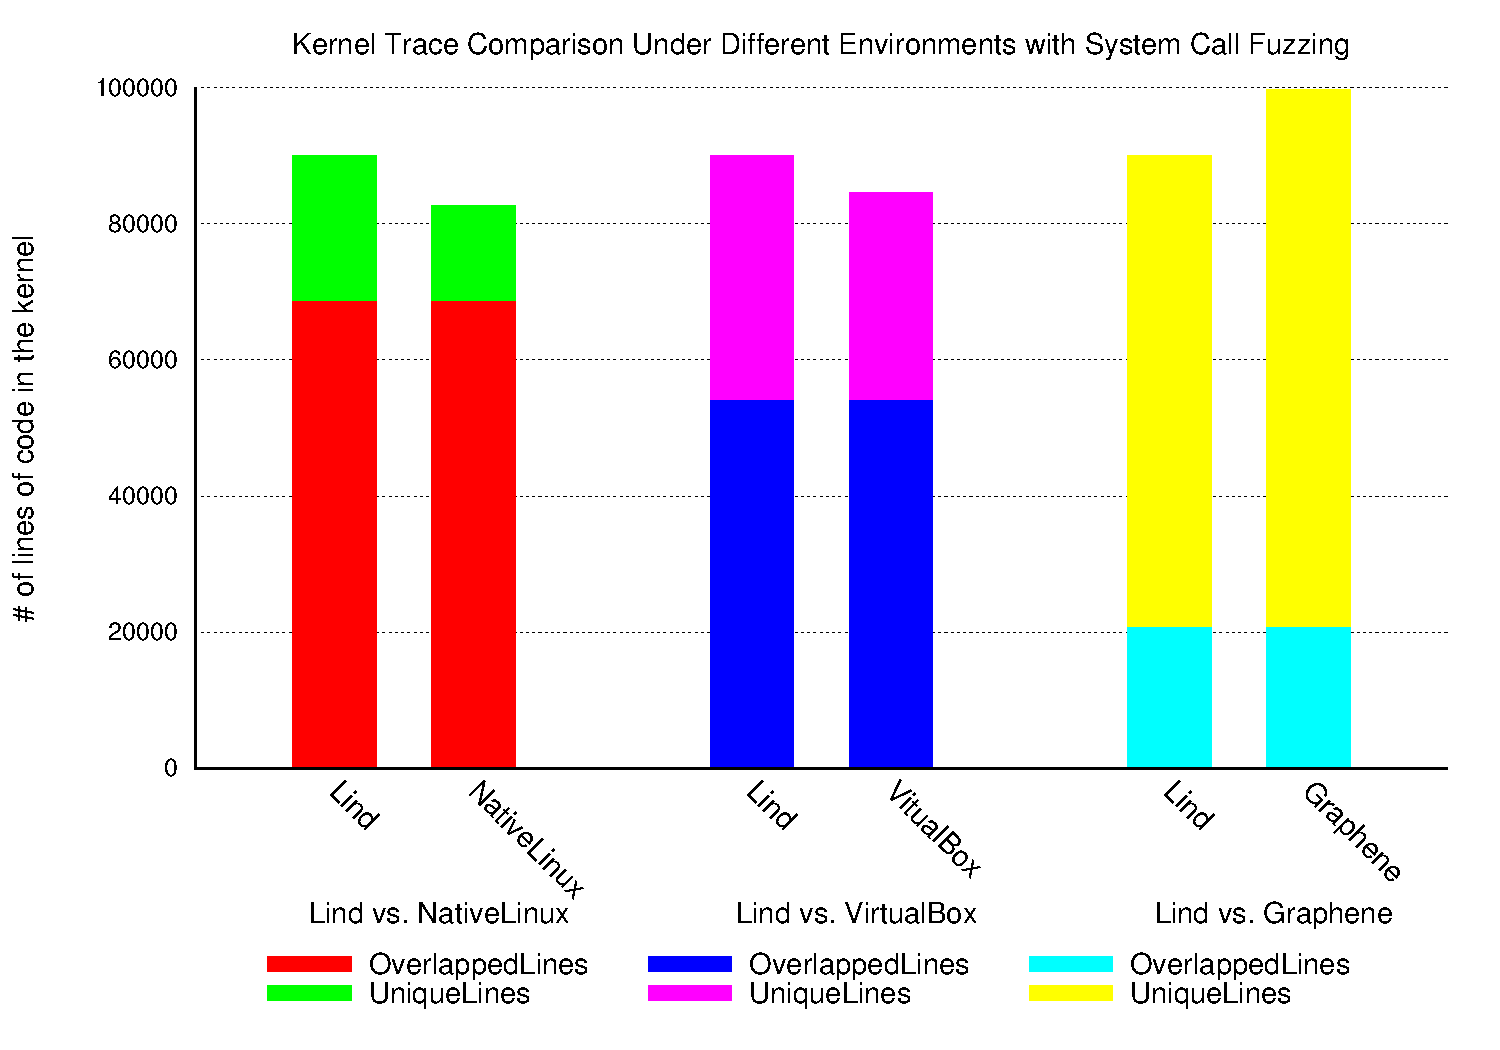
\includegraphics[width=1.0\columnwidth]{diagram/lind_ccs15_diagram_03.pdf}
\caption{Kernel Trace in Different Systems with System Call Fuzzing {\color{red}(The results are fake at the moment)} }
\label{fig:different_systems_systemcallfuzzing_trace}
\end{figure}

\begin{figure}[h]
\centering
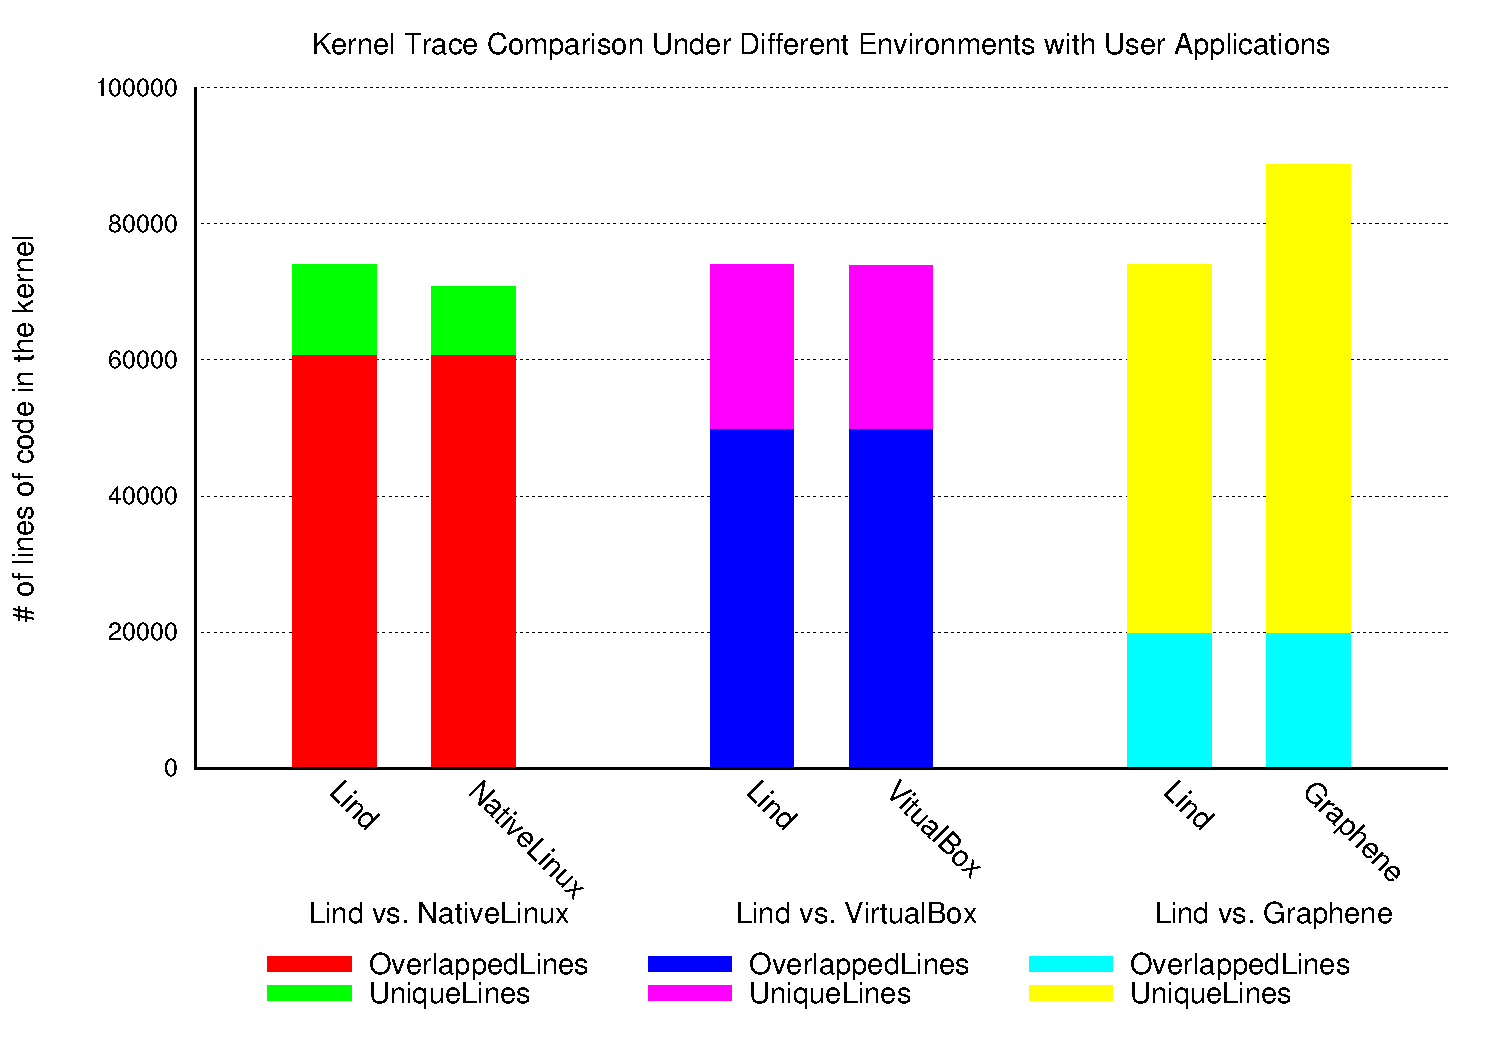
\includegraphics[width=1.0\columnwidth]{diagram/lind_ccs15_diagram_04.pdf}
\caption{Kernel Trace in Different Systems with Running User Applications {\color{red}(The results are fake at the moment)}}
\label{fig:different_systems_userapplications_trace}
\end{figure}

Now, we want to verify how likely it is to trigger kernel bugs in each of the environment.
We already had kernel trace generated by running system call fuzzing and user applications.
In order to check if kernel bugs might appear in those traces, we examined a list of 40 severe Linux 
kernel bugs (shown in Table 1), and identified the kernel paths involved in triggering each of the bugs.

The list of bugs we used in our experiments is shown in Table 1.

After examination of the bugs, we matched the kernel traces in different environments against the kernel traces generated 
by the bugs to verify if a bug might be triggered under each environment. 

The results for verifying which kernel bugs may be triggered under each environment is illustrated in Table 4.
From the results, we can see that Lind tends to provide stronger security than other systems.  

\subsubsection{Performance Evaluation}
Besides the security evaluation, we also did performance evaluation on running applications in each of the different environments.
The purpose of this performance evaluation is to show that although system like Lind is designed and built to provide stronger
security, it can also function well with reasonable overhead. 

Comparison results for the performance evaluation are shown in Figure 6.
The results show that the overhead of running applications in Lind is acceptable, compared with other systems. 
This suggests that systems designed and built using our metric can achieve the design goals, as well as function well in practice. 

\begin{figure}[h]
\centering
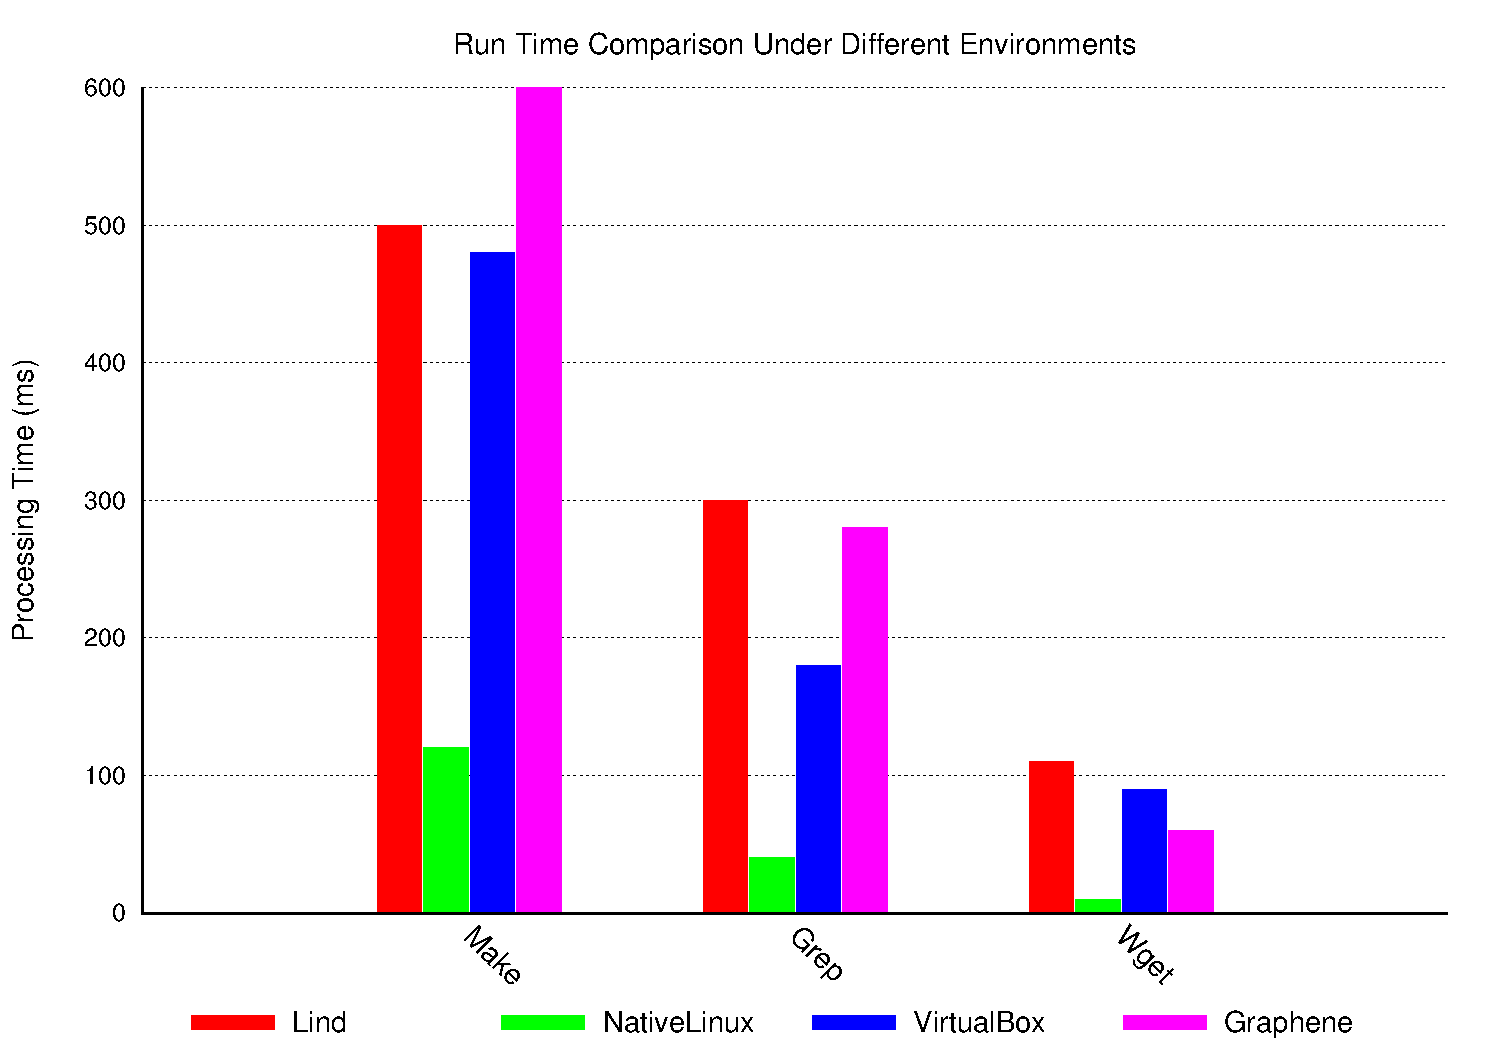
\includegraphics[width=1.0\columnwidth]{diagram/lind_ccs15_diagram_05.pdf}
\caption{Performance Evaluation Results {\color{red}(The results are fake at the moment)}}
\label{fig:performance_evaluation_results}
\end{figure}

\subsection{Conclusion}
Through our security evaluation and performance evaluation, we can see that 
Lind indeed achieved stronger security, compared against other systems.
Our metric is effective in creating new designs for building secure systems. 